% !TeX encoding = UTF-8

% 山二医入学与生活指南 © 2023 by LinkChou is licensed under CC BY-SA 4.0. To view a copy of this license, visit http://creativecommons.org/licenses/by-sa/4.0/

% 导入所需的package
\documentclass[a4paper,twoside,onecolumn,12pt,fontset=none]{ctexrep}
\usepackage{bxtexlogo,color}
\usepackage{fancyhdr,titlesec}
\usepackage{indentfirst,ulem}
\usepackage{float,graphicx}
\usepackage{multirow,booktabs,makecell,amssymb,array}
\usepackage{enumitem}
\usepackage[a4paper, hmargin=1.5cm, top=1.2cm, bottom=1.5cm, headheight=0pt, ignorehead]{geometry}
\usepackage[final=true, colorlinks, hidelinks, bookmarks, bookmarksnumbered=true]{hyperref}
\usepackage{datetime2}

% 重设定间距
\ctexset{
    chapter={
        beforeskip=0ex,
        afterskip=4ex
    },
    section={
        beforeskip=0ex,
        afterskip=0ex
    },
    subsection={
        beforeskip=0ex,
        afterskip=0ex
    }
}

% 重定义部分符号以免错误
\bxtexlogoimport{XeLaTeX}
\bxtexlogoimport{LaTeXe}

% 重定义文章字体
\setmainfont[BoldFont=Dream Han Serif CN W20]{Dream Han Serif CN W7}
\setCJKmainfont{Dream Han Serif CN W7}[BoldFont=Dream Han Serif CN W20]
\setCJKsansfont[BoldFont=Dream Han Serif CN W20]{Dream Han Serif CN W7}

% 段间距与行间距重设定
\setlength{\parskip}{.75ex plus 5pt minus 8pt}
\setlength{\lineskip}{.5ex plus 4pt minus 4pt}

% 页眉页脚
\pagestyle{fancy}
\fancyhf{}
\fancyfoot[C]{\thepage}

% 脚注格式
\renewcommand{\headrulewidth}{0pt}
\renewcommand{\footrulewidth}{0pt}
\renewcommand{\thefootnote}{\fnsymbol{footnote}}

% 列表样式重定义
\setlist[enumerate,1]{label=\arabic*.}
\setlist[enumerate,2]{label=(\arabic*)}
\setlist[enumerate,3]{label=[\arabic*]}
%\setlist[enumerate,4]{label=\{\arabic*\}}
\setlist[enumerate]{itemsep=0pt}

% 设置校徽背景命令
\newcommand\BackgroundPic{%
  \parbox{\paperwidth}{%
    \centering
    \vspace*{300pt}
    
\includegraphics[width=5cm]{background.pdf}%
  }
}

% 开始正文
\begin{document}

% 扉页

% 添加标题校徽背景图
\AddToHookNext{shipout/background}{\BackgroundPic}

% 题目
\title{%
\normalsize
\vspace{100pt}
{\Huge\textbf{山东第二医科大学指南}}\\[10pt]
(简称:\colored{171}{79}{36}{321指南})\\[30pt]
%{\large\textbf{\colored{59}{100}{220}{3.0.7}}}\vspace*{-25pt}}
{\large\colored{255}{0}{0}{320-Preview}}\vspace*{-25pt}}
\author{LinkChou\thanks{Compiled by \LaTeXe, CC BY-SA 4.0 LICENSE.\qquad%
        \uline{\href{Mailto:LinkChou@yandex.com}{Mailto: LinkChou@yandex.com}}\\
        \textbf{敬告:}\\
        \indent\indent 力薄才疏,不免舛误,敬请绳愆纠缪。具体内容均以学校官方为准,如有变更恕不另行通知。}
    \and 山东第二医科大学频道}
\date{\colored{36}{98}{105}{\CurrentCustomTime}}
\maketitle

% 脚注样式重设定
\renewcommand{\thefootnote}{\arabic{footnote}}

\tableofcontents
%chapter1
\chapter[简介]{简介}
\section[文章说明]{文章说明}

自豪地使用梦源宋体与梦源黑体进行排版。此外,如你所见,为避免文章引用混乱与格式在不同Office版本上的不断改变,本文章全部使用\TeX 语言写作,使用\XeLaTeX 引擎编译$pdf$文件,保证无论任何电脑都能获得相同的编辑体验(\sout{虽然入门门槛也高了许多})。

本文章原始大纲部分由“\textbf{潍坊医学院表白墙QQ频道}”提供,后经过“\textbf{\uuline{Mika}}”对原始主体部分进行全面重写与扩充而成,并保持积极的更新趋势,力求与学校实际保持同步。

而\textbf{\uuline{《潍医新生开学指南》}}是由“浮烟山小麻花”“vv”“花海”等人在本文的基础上进行重排版而成的新版本,通常以一年为周期进行版本更新。该版本相较本版,存在部分别字及过时内容。

\bigbreak
\textbf{\uuline{各位读者可视《潍坊医学院新生入学指南》为最新版本,《潍医新生开学指南》为现代化的主\\流发布版本。}}

本文以CC-BY-SA-4.0许可开源,仓库地址为\uline{\href{https://gitee.com/mikazo/guide_for_freshman}{Gitee}},欢迎各位同学参与项目的贡献!

本文\textbf{\uuline{最新版本下载地址}}为:\uline{\href{https://workdrive.zohoexternal.com/folder/sx5ijbbd2ad4d669c4c358d59fe314410aaf4}{Zoho Workdrive}}

\section[内容概要]{内容概要}

各位新同学可以在本文章中了解新生报到的各类要求,推荐准备的物品,学校的地图,宿舍的简要情况,周边的吃喝玩乐地点等。

虽然我们已尽力为大家总结,文章仍有不足之处,恳请各位同学斧正。

本文具体内容均以学校官方为准,内容如有变更恕不另行通知。
%地图
\chapter[地图]{地图}

\section[浮烟山校区地图]{浮烟山校区地图\footnotemark}
\footnotetext{原稿:校宣传部(整体地图)、临床医学院2021级学工办(教学楼地图);改图:LinkChou。}
\begin{figure}[H]
    \centering
    \caption[map_teach]{教学楼内部地图(浮烟山校区)}
    \vspace{1em}
    \includegraphics*[width=.9\textwidth]{教学楼_updated.jpg}
    \label{map_t}
\end{figure}

\newpage
\begin{figure}[H]
    \centering
    \caption[map_all]{整体地图(浮烟山校区)}
    \vspace{1em}
    \includegraphics*[width=\textwidth]{浮烟山整体地图.pdf}
    \label{map_a}
\end{figure}

\newpage
\section[虞河校区地图]{虞河校区地图}
\begin{center}
    制作中
\end{center}


% 入学准备
\section[入学准备]{入学准备}

\subsection[必要证件及物品]{\uuline{必要证件及物品}}
\begin{enumerate}
    \item \textbf{\uuline{录取通知书}}\footnotemark(必须带!!!)
          \footnotetext{录取通知书共两份,一份自行留存收藏,一份上交。}
    \item 身份证原件及其正反面复印件共4份(建议提前自行复印)
    \item 少量零散现金(100元左右即可)\footnotemark
          \footnotetext{校内各商店、超市、食堂支持微信、支付宝支付,部分支持云闪付;暂不支持数字人民币。}
    \item \textbf{证件照红、蓝、白底,1寸各6张、2寸各4张;以及各电子版}(开学后办理证件,如学生证、图书馆借阅证、社团会员证;各类手续,如团关系转接,学生档案转接,学生会入会申请表,体检报告等均需频繁使用;宿舍门禁系统登记时需要提供白底照片电子版)
    \item \textbf{\uuline{学生档案、团员档案}}(丢失或私自拆封需要补办后入学,切记勿忘勿丢勿拆!)
    \item \textbf{手机及配件}(充电器,充电宝,耳机,4~6根数据线〔长度在0.5m~1.5m均可〕)
    \item U盘(方便在校期间打印文件,避免异地登录QQ、微信泄露信息〔8G左右即可〕)
    \item \textbf{常备药物}(碘酒,创可贴,医用棉签,感冒灵,布洛芬,维生素,藿香正气水,止泻药,止咳药,跌打损伤药等)\textbf{\uuline{症状严重务必及时前往校医院就医,切勿自行用药耽误正规治疗}!}
\end{enumerate}

\subsection[选带证件及物品]{选带证件及物品}
\begin{enumerate}
    \item 户口本复印件1份,户口本本人页复印件4份\footnotemark
          \footnotetext{仅少部分院系要求报到时携带,具体要求以录取通知书为准。}
    \item 高考准考证、成绩证明页面的打印版\footnotemark
          \footnotetext{若录取通知书丢失,可通过以上材料证明身份。\label{lost_offer}}
    \item 相机以及配套储存卡、读卡器(⚠贵重物品,请妥存)
    \item \textbf{笔记本电脑}(班长团支、学生会及社团成员必需,其他同学按需)
    \item 平板\footnotemark
          \footnotetext{按照既往经验,有$\frac{1}{4}$左右的同学刷剧追番玩游戏的频率远超学习。}
    \item 备用眼镜、镜布及镜盒
    \item 病历本、住院证明等(仅因病无法参加军训者必备,详见\uline{\ref{exercise_unattend}})
\end{enumerate}

\subsection[推荐生活用品]{推荐生活用品}

\subsubsection[日用品]{日用品}
\begin{enumerate}
    \item 驱蚊花露水、风油精(严禁使用蚊香及电蚊香以防火灾)
    \item 洗面奶、护手霜、防晒霜等护肤品(不宜过多)
    \item 雨伞(2把,⚠易丢)
    \item 洗衣液/洗衣皂/洗衣粉及肥皂盒(建议带盖)、柔顺剂、消毒液
    \item 1.5L~2L的保温小水壶(冬天教学楼饮水机会上冻,提前接热水去自习好一些)
\end{enumerate}

\subsubsection[宿舍用品]{宿舍用品}
\begin{enumerate}
    \item 腰带(军训服尺码偏大)
    \item 袜子、鞋垫、内衣内裤和夏秋季换洗衣物(袜子至少10双,内衣内裤至少6套以免背阴面宿舍阴天无法及时晾干)
    \item 毯子或空调被(可以在录取通知书中查看本年度的配套被褥\footnotemark 价格,用料和质量都比较实在,据自身需求选订选带)
          \footnotetext{一般含夏被,冬被,褥子,枕芯,蚊帐,暖水瓶,塑料盆各一个;被套,床单,枕套,枕巾各两套;订购后会直接在开学时放到宿舍内,订购教程详见\uline{\ref{freshman_query}}。}
    \item 凉席、床垫\footnotemark(出汗严重或睡眠有特殊需求同学可自行选带)
          \footnotetext{宿舍床铺相对硬。}
    \item 蚊帐(已含于配套被褥中。注意:因四角支撑杆可能不全甚至全无,上铺的同学挂蚊帐比较困难;下铺相对方便。如有相关需求可前往校园周边五金店购买相关配件)
    \item 小锁(1把,用于锁柜子)
    \item \textbf{插排、转换器}(宿舍壁插数量少,刚需转换器;为确保安全,推荐购买公牛等知名品牌产品)
    \item 小台灯或手电筒(可用作考前熬夜学习或突然断电的应急措施)
    \item 衣服撑子、衣服夹子、粘钩(用于晾衣服,衣服撑子10个左右,夹子建议大小均有,被子夹6个,小夹子10个左右,粘钩有无均可)
    \item \textbf{几个干净的大型快递纸箱}(因学校的柜子比较脏且容易掉灰,可以先裁开纸箱子铺到自己的柜子里面再放置物品、衣物等以免弄脏)
    \item 樟脑球3个(不宜过多,放在柜子里以防生虫或衣物因为长期阴天而发霉)
\end{enumerate}

\subsection[学习用品]{学习用品}
\begin{enumerate}
    \item 书包(1个,仅用于上集体课)
    \item 手提袋子(1个,要求是耐脏便宜结实,当作书包用,仅用于实验课\footnotemark)
          \footnotetext{解释说明详见\uline{\ref{schoolbag}}。}
    \item 红蓝铅笔(中华牌很好,相对不容易断。医学实验课上全都是红蓝铅笔绘图)
    \item 订书机及订书钉或回形针(少用,\sout{但用一次头疼一次,因为很少有人有……})
    \item 美工刀,剪刀,胶水,双面胶,透明胶(拆快递、贴证件照常用)
    \item 记号笔(给课本封面写名字,课本也很容易丢)
    \item 4/6级英语考试单词书与练习题(4级6级基本都属于考研基础了,\sout{但愿大家能用上吧,不过\linebreak[3]二手书摊经常能买到全新的二手书,可见很多人都没怎么学})
\end{enumerate}

\subsection[相关注意事项]{相关注意事项}
\begin{enumerate}
    \item \textbf{\uuline{学校主要使用QQ进行联系以及官方通知的下发},且无“勤工俭学部”“兼职部”等学生会部门和社团,如遇类似组织推荐兼职请务必谨慎!}社团详情参见\uline{\ref{community_summary}},若不确定可联系本班班长或教师确认,谨防上当受骗!
    \item 安卓手机信号强度在学校停电时相对强(新生入学期间因违规电器导致跳闸频繁)
    \item 充电宝、充电器建议买名牌产品,杂牌劣质产品易出现用电事故;曾因杂牌劣质充电器短路导致多次宿舍全楼大跳闸
    \item 小台灯应当可充电或使用电池供电,以免停电期间无法使用
\end{enumerate}
%入学报到
\section[入学报到]{入学报到}

\subsection[地址与快递]{\uuline{地址与快递}}
\subsubsection[浮烟山校区]{浮烟山校区}
地址:山东省潍坊市潍城区望留街道宝通西街7166号山东第二医科大学浮烟山校区

快递地址:与学校地址相同

邮编:261053

取快递/寄快递:菜鸟驿站(宿舍楼\#12正北方约70米处,位置参见\uline{\ref{map_fuyanshan_holistic}}地图)

\subsubsection[虞河校区]{虞河校区}
地址:山东省潍坊市奎文区广文街道胜利东街4948号山东第二医科大学虞河校区

快递地址:与学校地址相同

邮编:261042

取快递/寄快递:北门菜鸟驿站(在校内,位置见\uline{\ref{map_yuhe_holistic}})、东门菜鸟驿站(在马路对面,校外)

\subsection[报到时间]{报到时间}
详见本人录取通知书

\subsection[浮烟山校区报到流程]{浮烟山校区报到流程}
\begin{enumerate}
    \item \textbf{\uuline{在“山东第二医科大学学生之家”公众号进行预报到},并查询自己的宿舍编号,学号,班级,院系等信息}\footnotemark(教程详见\uline{\ref{freshman_query}})
          \footnotetext{公众号查询入口开放日期约为8月20日前后,每年不一。}
    \item 通过学校通知、各级学生会、贴吧或频道创建的官方群内指引或者等待各位带班学长学姐加好友后进入班级群\footnotemark
          \footnotetext{若未能寻找到自己的班级,也可在报到时通过带班学长学姐加入班级官群。}
    \item 根据\uline{\ref{goto_school}}前往山东第二医科大学(浮烟山校区)北校门,在志愿者\footnotemark 的带领下先前往宿舍一楼(各宿舍楼位置见\uline{\ref{map_fuyanshan_holistic}}),在宿管阿姨处领取宿舍钥匙并登记信息
          \footnotetext{注意,\textbf{男女宿舍不互通},请尽量找相同性别的志愿者帮忙。}
    \item 暂时放置行李物品,进行物品的初步整理
    \item 携带本人身份证件、录取通知书\footnotemark 及中性笔一只,前往杏林路D区方位(位置参见\uline{\ref{map_fuyanshan_holistic}})
          \footnotetext{录取通知书丢失处理办法见此\uline{\ref{lost_offer}}。}
    \item 在公安设置的身份核验处查验自己的身份证\footnotemark 信息
          \footnotetext{身份证丢失或失效请立即在学校110警务处申请临时身份证。}
    \item 根据杏林路西侧的指示牌寻找自己班级的带班学长、学姐报到并签字,他们将指引你完成接下来的报到流程\footnotemark
          \footnotetext{如果前往学校的时间过晚或未能及时购票,可前往学院官网,通过官网最下方的联系方式咨询本学院教师解决方案;按照往年惯例,未能及时登记报到的同学会统一补齐相关记录。}
    \item 返回宿舍或前往菜鸟驿站领取并整理自己的被褥等个人物品
\end{enumerate}
%宿舍
\chapter[宿舍及校园环境]{宿舍及校园环境}

\section[整体情况介绍]{整体情况介绍}
\subsection[浮烟山校区]{浮烟山校区}
\begin{enumerate}
      \item 绝大多数的宿舍为6人间,上下床(各床铺靠墙侧均有1插座,可接插排),配备桌子(桌洞8个)一张,书桌(理论可坐3人但空间紧张,常2人,含6个小书架)一张,有柜子(常为8个),垃圾桶,洗漱池,空调,电风扇,暖气片,烟雾报警器等宿舍基本设施
      \item 柜子\footnotemark 一般为8个,6人各选一个柜子,剩下两个公用
            \footnotetext{空间参数大致如下:宽62cm,高59cm,深97cm(各有1~2cm误差)。}
      \item 具有独立卫生间
      \item 部分女生宿舍的卫生间内有浴室,可直接在卫生间内淋浴;其他同学可以在本楼层小公共澡堂(有2个毛玻璃隔间,有门帘,无需预约)或者一楼的大公共澡堂(不透明隔间,有门帘,需软件预约)洗澡(教程见此\uline{\ref{shower_software_f}})
      \item 洗衣机位于每层楼的公共洗漱间内(教程见此\uline{\ref{washing_machine_f}})
      \item 烘干机位于每栋楼1层公共洗漱间内(教程见此\uline{\ref{dry_machine}})
      \item 吹风机位于每层楼的公共厕所旁(教程见此\uline{\ref{hair_drier}})
      \item 宿舍楼06:00开门,23:00关门;23:00断电(\textbf{每周六、考试月和每年9月的第一个星期除外});大一期间,院系学生会每周不定时抽查是否存在夜不归宿情况
      \item 空调采用单独线路供电,不受断电熄灯控制(全楼断电等特殊情况除外),需另外缴费(使用教程参见\uline{\ref{air_control}})
      \item 使用门禁系统刷脸进出宿舍
      \item 宿舍楼提供免费的100℃开水\footnotemark,若对饮水水质要求不高也可直接饮用;否则请前往大学生服务中心〔简称“大服”〕打水处(位置参见\uline{\ref{map_fuyanshan_holistic}})付费接取纯净水
            \footnotetext{饮水机每层一个,位于公共洗漱间内;为自来水烧开;熄灯后停止供应。推荐用于泡面、洗衣、泡脚等用途。}
      \item \textbf{\uuline{宿舍单个插座限电400W,超限将导致全楼停电}}
      \item 除跳闸断电等特殊情况外,其余时间段均有4G及5G信号覆盖,延迟波动较大(15~999$^+$㎳),平均网速1.5~5㎆/s
\end{enumerate}

\subsection[虞河校区]{虞河校区}
\begin{enumerate}
      \item 本科宿舍无阳台,无独立卫生间,面积稍小于浮烟山校区
      \item 虞河校区无操场,仅篮球场一个;无完备实验室
      \item 宿舍不断电但限制功率
      \item 饮水机每层一个,为自来水净化后烧开,24小时供应
      \item 学校洗浴中心在3号楼负1层(男浴室内共14隔间),各宿舍楼内不可洗浴,教程见\uline{\ref{shower_software_y}})
      \item 宿舍楼06:00开门,23:00关门
      \item 东门06:00开门,23:00关门;\textbf{北门全天开放}
      \item 其余与浮烟山校区基本相同
\end{enumerate}


\section[住宿注意事项]{住宿注意事项}
\subsection[浮烟山校区]{浮烟山校区}
\begin{enumerate}
      \item \textbf{\uuline{宿舍以专业为单位进行随机分配宿舍楼、班内宿舍按姓氏顺序分配,与录取分数无关}}
            \label{random_allocation}
      \item 是否自带被褥等可按照个人需求决定\footnotemark
            \footnotetext{新生军训期间对于床单的颜色等具有特别要求,详见录取通知书相关说明。}
      \item 宿舍门禁系统将在开学军训期间进行人脸录入,\textbf{\uuline{切忌美颜过度,否则无法识别}}
      \item 无特殊情况\textbf{禁止自挂床帘},特殊需求请找导员开具证明
      \item 宿舍内备有烟雾传感器,\textbf{吸烟将引发报警\footnotemark}
            \footnotetext{若烟雾报警器报警,请立即联系宿舍管理人员或保卫科核实。}
      \item 床上桌等类似的东西建议到学校实际生活1个月以后再决定是否购买(大部分人都用不到,少数同学用来打游戏,\sout{然而身体在床上缩着打游戏超级难受};更少一部分同学用其学习,\sout{该现象\linebreak[3]比彩色大熊猫更加罕见})
      \item 宿舍单个插座的功率限制400W\footnotemark,\textbf{\uuline{吹风机,锅,电暖宝,电水壶,热得快等高功率电器均严}}\linebreak[3]\textbf{\uuline{禁使用},否则将引起宿舍全楼停电};宿管不定期来查,若被发现将被没收并通报批评、检讨
            \footnotetext{如果接了一个插排,插排的总功率不能超过400W,例如一个67W的手机充电器和2个175W的游戏本电脑就立马跳闸了。}
      \item 如需装修宿舍,可通过参加学校统一开展的\textbf{“宿舍装扮大赛”}\footnotemark 以对宿舍进行小幅调整
            \footnotetext{大赛禁止外来装修人员入校、禁止私改电路,详情内容见开学后下发的参赛要求。}
      \item 背阴面宿舍的阳台相当于摆设,\textbf{推荐在楼下晾晒衣物},若只靠阴干,很容易发霉发臭;向阳面无此困扰
      \item \textbf{一旦离开宿舍必须关灯关电,若插排未拔将被没收并扣分}
      \item 禁止将正在持续充电的手机、充电宝直接置于被子等密闭、空气无流通的环境中,极不推荐直接将笔记本电脑置于被子上使用,严重影响散热且有着火风险
      \item \textbf{\uuline{为保证他人睡眠,熄灯后严禁使用台灯、手电筒在宿舍内继续学习;更不要制造噪音!}}\footnotemark
            \footnotetext{很多同学难以入睡且睡眠浅,小动静或急速的明暗变化就能被惊醒,请大家务必相互尊重、相互理解。}
      \item 如遇宿舍公用物品(如门锁,门轴,玻璃窗,灯管,水龙头,下水道等)损坏,请直接报修(教程见此\uline{\ref{repair_report}})
      \item 宿舍一层有便民驿站(含针线包、打气筒、简易医药箱),即用即还
      \item 雨伞不得长时间放置于宿舍门外,避免影响正常通行
      \item \textbf{严禁在23:30以后使用洗衣机、烘干机、吹风机或洗澡。}
\end{enumerate}

\subsection[虞河校区]{虞河校区}
\begin{enumerate}
      \item 学校为全开放式校园,允许社会人士出入,\textbf{请务必锁门关窗,谨防小偷}
      \item 宿舍隔音效果较差,\textbf{严禁在中午、夜晚等休息时间段打篮球}
      \item \uuline{\textbf{严禁在走廊大声喧哗}}
\end{enumerate}

%chapter6
\chapter[军训]{军训\vspace{-2em}}
\section[军训概况]{军训概况}
\begin{enumerate}
    \item 军训时间:3周,报到后马上开始
    \item 内容\footnote{不打靶、不摸枪;少数同学会参与战术方阵,女生有擒敌拳。}:站军姿,蹲下,跨立,齐步走,原地踏步,齐步跑,踢正步,坐马扎
    \item 地点:多数在杏林路树荫下军训(一般晒不着,但仍然建议多备防晒霜)
    \item 教官:通常由退役复员的学长学姐担任,也有部分现役武警(或现役解放军)组成,一般年纪都不是特别大,大部分是90后
    \item 着装:穿着统一的军训套装\footnotemark
          \footnotetext{统一收费,支持现金及扫码。包括T恤,外套,裤子(很肥),腰带(扎在外套外面,需另备一条腰带以免掉裤子),鞋子(底薄、磨脚,推荐鞋子大一号多垫几双鞋垫)和马扎(军训完马扎不要扔,考试月背书的时候很好用)。}
    \item \textbf{如果因为身体原因不能参加军训,需要提前拿病历、住院证明等材料前往校医院}(位置参见\uline{\ref{map_a}})开具证明\label{exercise_unattend}
    \item 若出现身体不适要及时向教官报告,较严重的可申请前往校医院或附属医院进行详细检查
    \item \sout{如果顺拐和左右不分情况极其严重的,可以早早申请成为“飞虎队”\footnotemark 的一员}
          \footnotetext{谐音梗,音同废物队;是对顺拐同学的无恶意调侃。}
    \item 特点:军训期间时间紧、任务重,少有可以自由安排的时间
    \item 注意:\textbf{\uuline{可能出现长时间阴天}},因此推荐多带袜子,内裤,内衣,T恤以避免一件衣服穿一周(\sout{熏死啦,想想就头大})、袜子晾干以后变得硬邦邦的(\sout{长蘑菇了都})的悲伤结局
\end{enumerate}

\section[军训作息时间表]{军训作息时间表\footnote{以往届作息为例,具体以各学院安排为准。}}
\vspace{-1.5em}
\begin{table}[ht]
    \centering
    \begin{tabular}{|c|c|c|c|}
        \hline
        5:30        & 起床 & 12:30-14:00 & 午休  \\
        \hline
        6:00-7:00   & 早操 & 14:00-17:30 & 集训  \\
        \hline
        7:00-7:50   & 早餐 & 17:30-18:30 & 晚餐  \\
        \hline
        7:50-11:00  & 集训 & 18:30-21:30 & 晚自习 \\
        \hline
        11:00-12:30 & 午餐 & 23:00       & 熄灯  \\
        \hline
    \end{tabular}
    \vspace{-0.5em}
    \caption[exercise_time]{军训作息时间表}
\end{table}

%chapter7
\chapter[学习方面]{学习方面}
\vspace{-1em}

\section[学分]{学分\footnotemark}
\footnotetext{因不同学制、学院、年级要求各不相同,本图仅以2021级临床医学院临床医学系普通5年制本科为例,依照教务处\uline{\href{https://jwch.wfmc.edu.cn/2022/0916/c5343a107934/page.htm}{《潍坊医学院本科专业人才培养方案(2021版)》}}制作,具体内容参见学生手册相关章节和教务处官网说明,如有变更恕不另行通知。}
\vspace{-1em}
\begin{table}[ht]
      \centering
      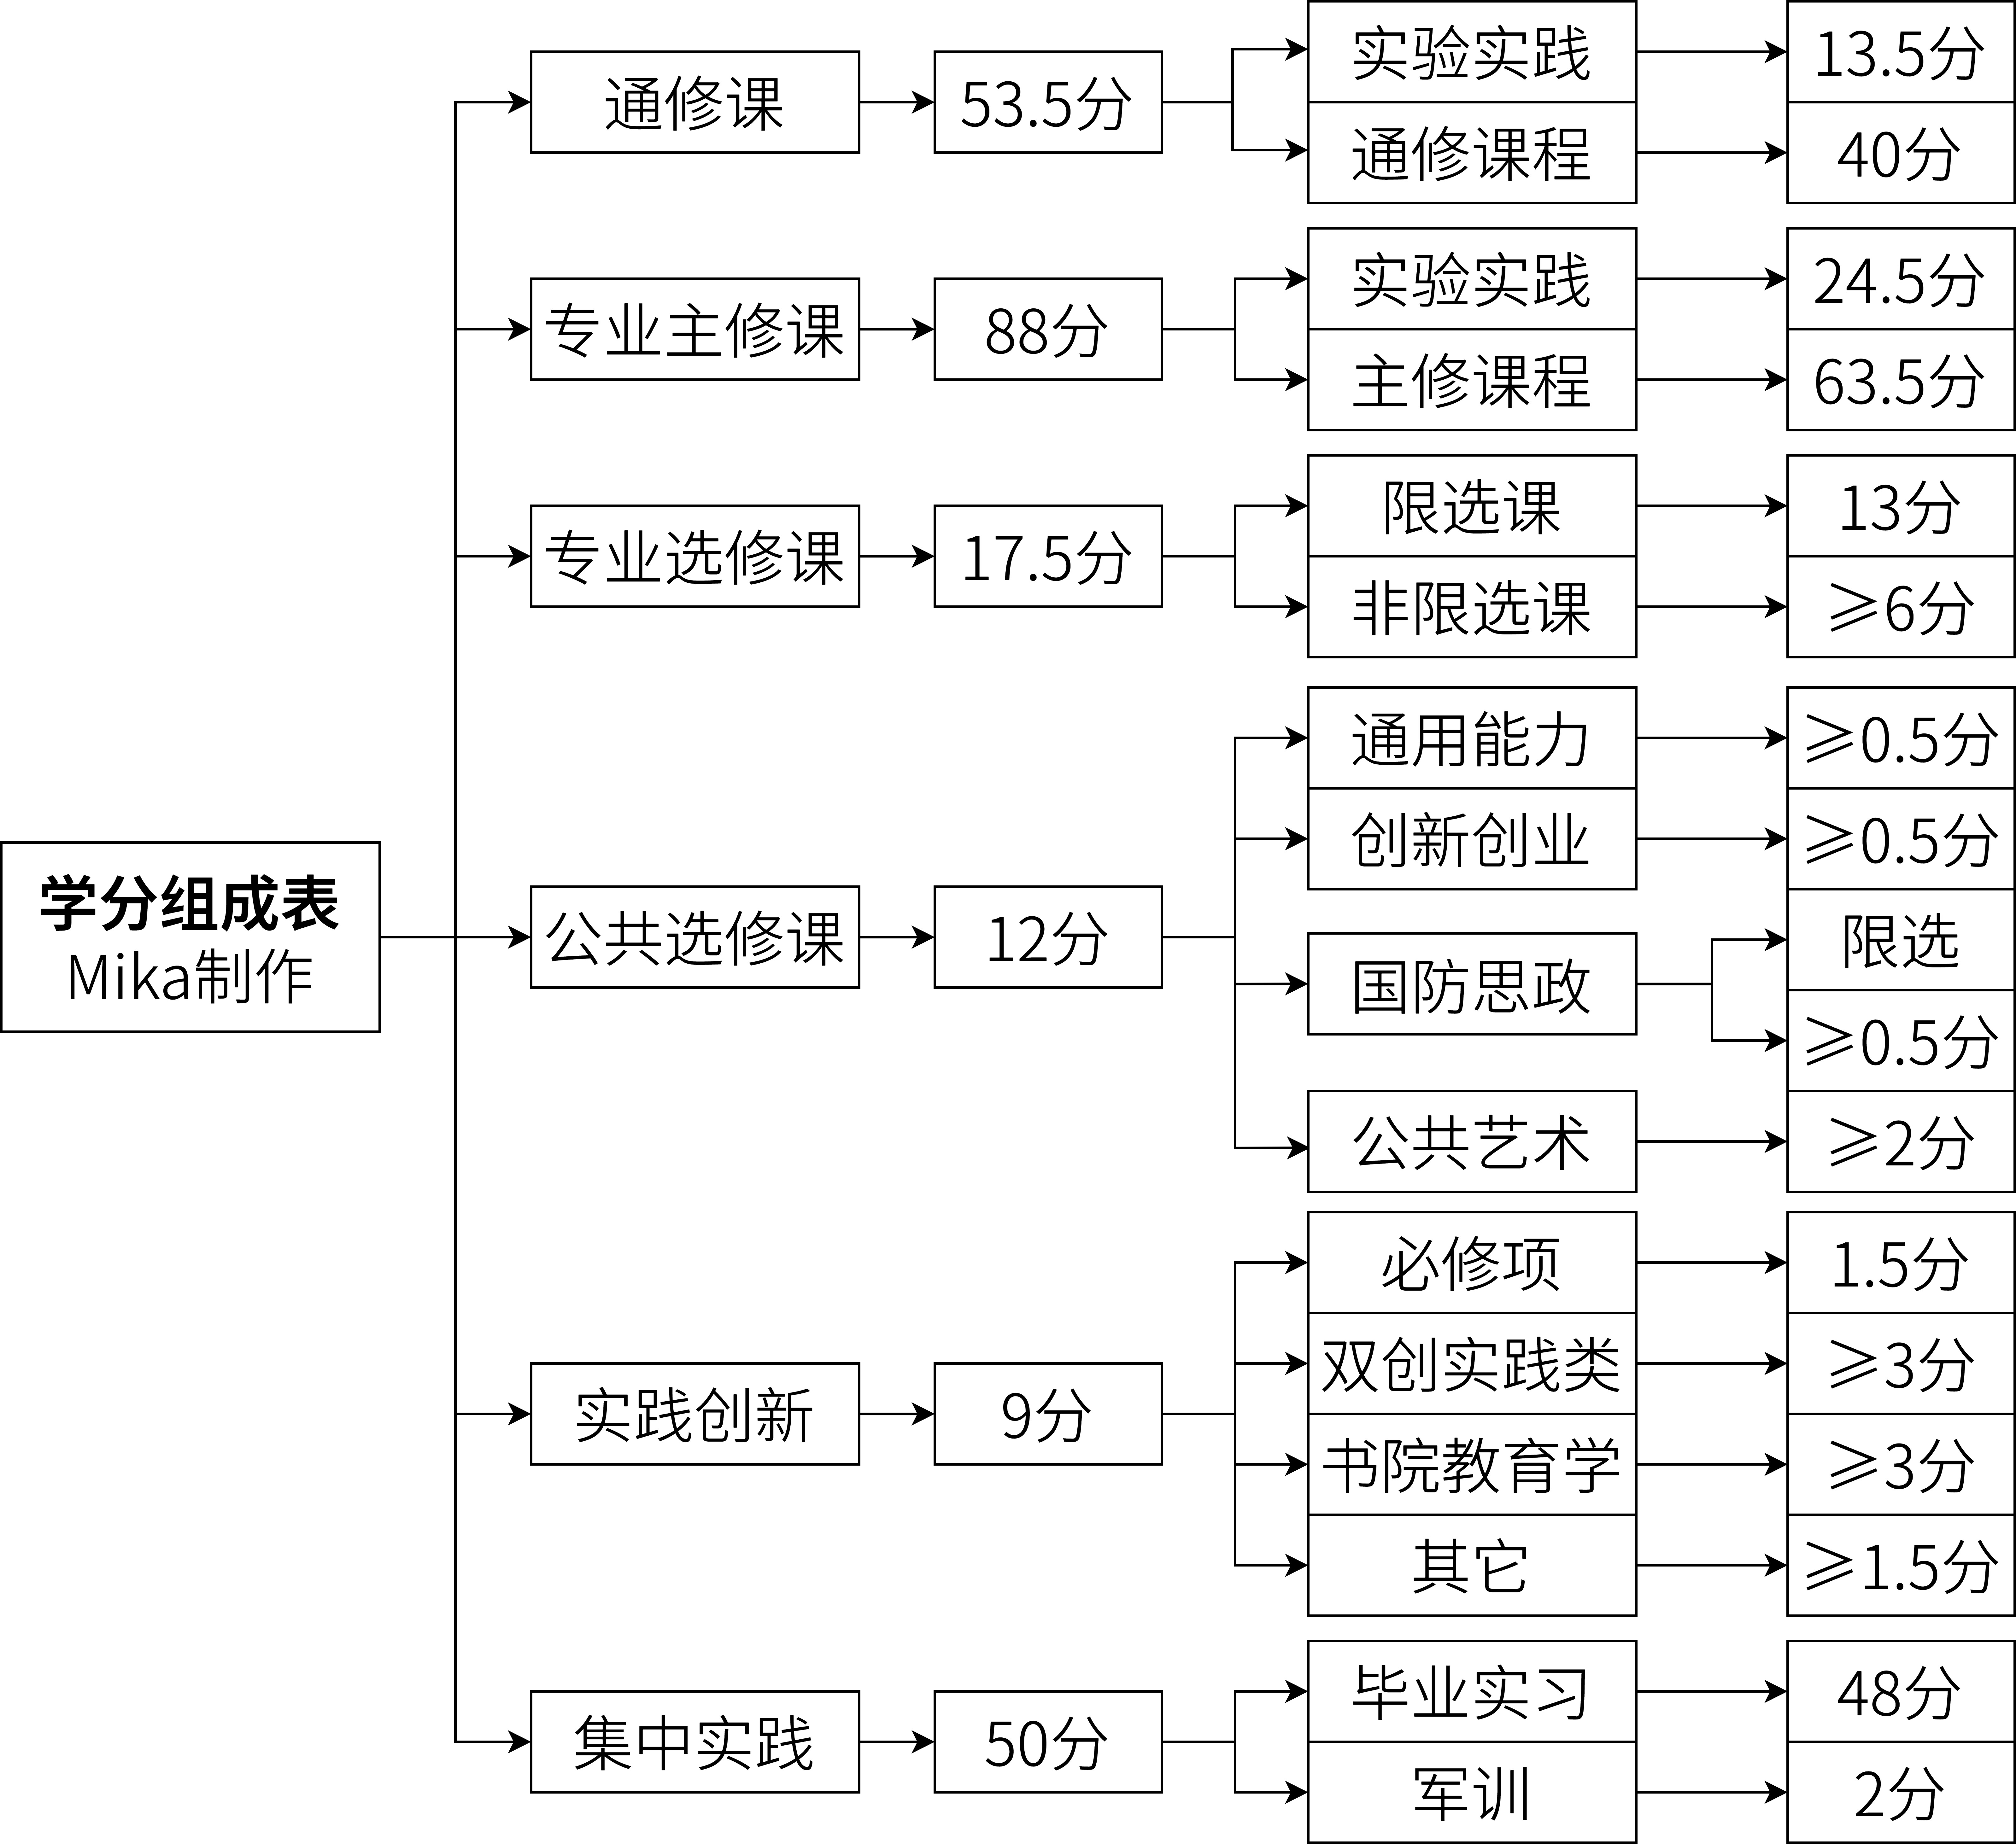
\includegraphics[width=\textwidth]{学分.jpg}
      \vspace{-1em}
      \caption[学分组成示意图]{学分组成示意图}
      \label{score}
\end{table}

\newpage

\section[关于选修课的补充说明]{关于选修课的补充说明}
\begin{enumerate}
      \item 选修课分专业选修和公共选修两大类(详见\uline{\ref{score}}),\textbf{推荐在大一全年、大二上学期的把各类选修学分全都修满},这样就不用在后面学业愈重的情况下兼顾选修课的学习了,可以专心针对专业课程进行深入学习
      \item 专业选修课有限选和非限选之分,限选的课程无需操心,教务系统会自动选课,只需要保证非限选的课程学分达标即可
      \item 公共选修课每一类都要选至少一门,且需要满足总分,其中部分类别还有额外要求(详见\uline{\ref{score}}),国防教育类有国家限选课程(到时候看具体通知,会说的很明白的)
      \item 公共选修课有一部分是在教室上的,还有一部分是线上课程(使用“知到”app进行学习,大多数有平时分,不能突击),可以根据自己的实际情况选择\footnotemark
            \footnotetext{一般来讲线下课好过,每星期去一次教室听听课就行,结课考试也很简单;但是线上课随时都能刷课,刷完课考完试就不用每周都去听课了,根据自己的需求选择。}
      \item \textbf{\uuline{公共选修课联盟的公共选修课程不算学分、不收学费}}
\end{enumerate}

\section[特殊说明]{特殊规定说明}
\begin{enumerate}
      \item \textbf{\uuline{大一不组织参加四六级,大二才能报名四六级考试}}
      \item \textbf{\uuline{转专业}\footnotemark:}
            \footnotetext{依据教务处2023年5月31日发布的\uline{\href{https://jwch.wfmc.edu.cn/2023/0531/c2593a117986/page.htm}{《潍坊医学院2023年普通全日制本科学生转专业工作方案》}}简化,具体规定详见链接。今后如有变动,以学校官网为准。}
            \begin{enumerate}
                  \item 需满足以下条件:
                        \begin{enumerate}
                              \item 取得学籍的普通全日制一年级本科在校生
                              \item 未受处分、思想过硬、符合体检要求
                              \item 第一学年必修课和专业限定选修课平均成绩在本专业排名前30\%,且未挂科
                              \item 公费医学生,春季高考,第二学士学位,贯通培养学生等以特殊招生形式录取的学生;国家有相关规定或者录取前与学校有明确约定的,不得申请转专业
                        \end{enumerate}
                  \item 流程:
                        \begin{enumerate}
                              \item 考试科目为思政、英语、数学,比例为1:1:1,考试时间150分钟,总分为150分
                              \item 核算学生第一学年学习成绩并公示各类数据
                              \item 8月27日开始报名
                              \item 8月31日组织考试
                              \item 9月1日-5日公示录取名单\footnotemark
                                    \footnotetext{按照“分数优先,遵循志愿”的原则进行录取。}
                              \item 9月6日-7日报到
                        \end{enumerate}
            \end{enumerate}
      \item 关于奖学金\footnotemark:本校有国家奖学金、校长奖学金、校级3等级奖学金等
            \footnotetext{请注意,目前学校仅能通过本人身份开通的,已开户的,账户已激活的,无异常的,工商银行的储蓄卡发放奖学金,详情政策可咨询学校财务处。}
      \item 新生开学考试\footnotemark 的内容为高中英语、高中数学,旨在让各位同学收心
            \footnotetext{按照往年惯例,不公布具体成绩。}
      \item \textbf{关于档案填写:}开学以后需要大量填写各类表格,如果你听到“入档”这两个字时需要格外注意,入档资料具有不能涂改、不能标记、不能修正的特性,因此严禁使用修正液或修正带对其涂改(涂改修正后立即作废)。填表时务必确保各类时间填写正确、与原始档案一致。此外,建议初次填写时使用铅笔轻轻填写,待负责人确认无误后方可擦除后使用黑色中性笔或中油笔填写(入档纸张为特殊A4纸,与正常A4纸相比厚、重、滑,难以自行复印请注意)
      \item 挂科与补考、重修:因各年级、院系要求不一,详见学校下发的学生手册
      \item \textbf{关于实验课与实验服:在实验课上课时务必按要求正确洗手并佩戴头套、口罩、手套,着实验服,\uuline{严禁任何人在任何地点(尤其是餐厅)着实验服}!因在实验室中需频繁接触实验动物、微生物,\uuline{极其推荐将实验课书包与普通课书包分开}!}
            \label{schoolbag}
\end{enumerate}

\section[早操与晚自习]{早操与晚自习}
\begin{enumerate}
      \item 早操时间一般为6:00-7:00,晚自习时间通常为18:30-21:00,教室22:00关闭
      \item 早操与晚自习贯穿整个大一\footnotemark,并且跑操与晚自习均有院系学生会不定时进行抽查人数是否到齐等指标,最终结果计入班级综测(详见下文\uline{\ref{class_evaluation}})的评分
            \footnotetext{按照惯例,麻醉专业无早操,只需要大一、大二早晨七点签到。}
\end{enumerate}

\section[班级综测]{班级综测}
\label{class_evaluation}
\begin{enumerate}
      \item 班级综测是用于考核各班表现的评判指标和分配实习点的依据\footnotemark,每学期计算一次,截至见习
            \footnotetext{以截至见习之前的各学期平均班级综测成绩计算班级排名,公费班级根据本年级政策进行。}
      \item 由班级平均成绩、比赛类、表彰类等类别构成,详见学生手册(各年级要求不一)
      \item 班级综测直接决定本班级同学后期学习和生活所在的医院规模、等级和生活条件(例如宿舍有无空调、暖气、洗衣机,是否提供插座,是否有早操和晚查寝\footnotemark 等),请大家务必重视
            \footnotetext{这意味着能否在外租房居住。}
\end{enumerate}

\section[学长学姐的特别叮嘱]{学长学姐的特别叮嘱}

进入大学之后,很多人都会在学习上松懈。的确,数十载的苦读,为的就是一朝踏进大学“万事无忧”,然而我们真的可以在大学里肆意放纵吗?

进入大学之后,你或许也会听到无数“好心的学长”告诉你:玩吧,大一不玩,以后就没时间玩了;等开了专业课,学习任务越来越重,就没有玩乐的时间了;没有挂过科的大学生活是不完整的。

于是你心动了、放纵了,上课不怎么去了,课本不怎么看了,眼睛盯着各种游戏和活动移不开了。然后毫无疑问,期末考试你挂科\footnotemark 了。
\footnotetext{一次挂科影响深远!让你从此远离所有转专业、奖学金以及大型表彰;考名校的研究生也会有更大的竞争压力。}

所以啊,亲爱的新生们,千万不要把学习放下了。虽然在大学与高中截然不同,有多样的活动、宽松的环境……但是你来到大学的初心是为了学习更多的专业知识,\sout{也可能是更高的工资},但无论如何,知识都是大家前往更高的工资、更好的工作环境、更优秀的公司的敲门砖。所以,认真学习吧,学习才是真正的\textbf{“捷径”}。然后,在保证学习时间和质量的前提下,再去做其他的想做的事。

%安全
\chapter[安全方面]{安全方面}

\section[用电安全]{用电安全}
\begin{enumerate}
    \item 使用安全的充电器、充电线、插排
    \item 如遇空调、电灯、电风扇等器具出现短路、跳闸、停电等现象时切勿自行维修,请按照\uline{\ref{repair_report}}教程处理
    \item 切勿在宿舍使用冰箱(断电且宿管检查),\textbf{\uuline{如果各位同学需要冷藏保存药物(如胰岛素等),请\\前往校医院或大服2楼的药店处}}(地点参见\uline{\ref{common_locations}}),具体收费情况请咨询相关人员
    \item 切勿私改电路,如确有需要,应提前向宿管及公寓管理委员会\footnotemark 报备并获得相应许可
          \footnotetext{位于2号公寓南门处。}
    \item 宿舍人走灭灯,无人则关电、切断插座电源
\end{enumerate}

\section[防火安全]{防火安全}
\begin{enumerate}
    \item 切勿使用蚊香以免发生火灾
    \item 切勿在宿舍内烹饪,禁止在宿舍使用各类燃气灶、固体酒精便携灶等易燃易爆危险品
    \item \textbf{禁止在宿舍内吸烟},若实在无法抑制请前往本楼层公共厕所或在宿舍外吸烟完毕后再进宿舍
    \item 请妥善保管打火机、打火石、镁条、火柴等易燃物
\end{enumerate}

\section[出行安全]{出行安全}
\begin{enumerate}
    \item 学校周边基础设施尚在完善建设过程中(\sout{属实是兔葵燕麦、雨井烟垣}),且频繁有货车高速通过。如无特殊情况,\textbf{尽量不要骑公共自行车或者电动车去市里}(泰华城)等,推荐乘坐71路公交车(预计行程30分钟左右)或打车前往
    \item 货车转弯盲区大,极其容易发生安全事故,在等红绿灯时请务必远离“站立禁止区域”
    \item 乘坐出租车(尤其是拼车时)请妥善保管自身财物;如遇失窃请尽快报警,避免正面冲突(谨防持刀伤人)
    \item \textbf{\uuline{严格遵守交通规则,仔细观察周围情况,切忌边看手机边前进,切忌闯红灯}!}
\end{enumerate}

\section[食品安全]{食品安全}
\begin{enumerate}
    \item 如果在餐厅吃坏了肚子或者发现食物质量问题,可前往餐厅一楼东北角的值班室寻求工作人员的帮助
    \item 出现急性腹泻、血便、米泔水样腹泻等情况请尽快前往校医院就诊,切勿拖延
\end{enumerate}

\section[防诈骗及其他注意事项]{防诈骗及其他注意事项}
\begin{enumerate}
    \item \textbf{\uuline{校园贷毁一生,远离高利贷}!}
    \item \textbf{\uuline{杜绝黄赌毒!不要高估自己的意志力}!}
    \item \textbf{刷单就是诈骗!}
    \item 不要贪小便宜乱扫码,信息泄露吃大亏!
    \item \textbf{\uuline{在正式开学、由带班学长学姐拉入年级的官方QQ群之前,所有的主动拉人入群的各类“通\\知群”“官方群”“学生公告群”等均不可信}!}
    \item 如果碰到一些人自称是市场营销专业、经商专业的,需要卖笔卖本子\footnotemark (总之是找人要钱)才能完成期末考试的,千万不要相信!可以直接联系保卫处
          \footnotetext{一支批发0.1$¥$的笔卖10$¥$呢,比百乐斑马这种外国牌子都贵,利润高达10000\%……}
    \item 女生晚上尽量不要独自前往人烟稀少的地方,尤其是西门附近的桃李路等
    \item 谨防诈骗,\textbf{学校永远不会以教务处、学工办的名义,以邮件表格或短信链接的形式通知填写银行卡号和取款密码!}绝对不要相信以“更新银行卡信息”、“填表申请助学金”为由窃取个人资金密码的骗局!如果不确定消息是否属实请致电本班班长,班主任或学工办老师确认
    \item 各位家长在向学生转账时应确认钱款具体用途、打款账户是否正确,同时应当电话询问是否属实,谨防盗号诈骗
\end{enumerate}

%chapter9
\chapter[衣食住玩与生活]{衣食住玩与生活}
\section*{特别声明}
\begin{enumerate}
    \item 本文中所有\textbf{“大服”},均为\textbf{“大学生服务中心”}的习惯性缩略称呼;
    \item 本文中所有\textbf{“南街”},均为\textbf{“汇金街”}的习惯性缩略称呼。
\end{enumerate}
\section[衣]{衣}
\begin{enumerate}
    \item 大服的2、3层均有服饰商店可自行选购衣物
    \item 推荐网购,也可乘71路等公共汽车前往大型商超购置
    \item 部分院系提供自愿的系服购买服务,详见各院系通知
\end{enumerate}

\section[美食与生活]{美食与生活}

\subsection*{注意}
\begin{enumerate}
    \item 因文章篇幅原因,本指南仅罗列了同学们提及次数较多的食物或店铺,未能全部列出敬请谅解;
    \item 下列提及的店铺(食物)均按照空间顺序排列,与好吃程度无关;
    \item 所用名称为同学习惯性称呼,括号内为特别提醒。
    \item 上标“㊐”的店铺夏季约6:00开始供应(冬季约6:30);
    \item 上标“㊰”的店铺营业时间最晚可至22:30,其余均在18:30左右停业。
    \item 奶茶/咖啡店、超市、水果店等单独说明。
\end{enumerate}

\subsection[大服]{大服}
大服有大量商家提供多种食物,大部分的价格较食堂稍高。
\begin{table}[H]
    \centering
    \begin{tabular}{|c|c|c|c|c|c|}
        \Xhline{1.2pt}
        \multirow{3}{*}{1层}  & \multirow{2}{*}{内}                              %
                             & 金小麵$^{㊐}$(锅贴)                 & 自选菜             %
                             & 陕西面馆                          & 馋嘴鱼             \\
        \cline{3-6}
                             &                                                 %
                             & 新疆炒米粉                         & 肠粉              %
                             & 肉夹馍$^{㊰}$                     & 冒菜              \\
        \Xcline{2-6}{0.8pt}
                             & 外                                               %
                             & 烧烤$^{㊰}$                      & 砂锅$^{㊐}$(火烧|豆脑) %
                             & 大饼卷一切$^{㊰}$                   & 速食主义$^{㊐}$      \\
        \Xhline{1.2pt}
        \multirow{2}{*}{-1层} & \multirow{2}{*}{$\backslash$}                   %
                             & 兰李于                           & 自选菜             %
                             & 酸菜鱼                           & 螺狮粉             \\
        \cline{3-6}
                             &                                                 %
                             & 烤鸡架                           & 宽巷面馆            %
                             & 馋嘴鱼                           & 略               \\
        \Xhline{1.2pt}
    \end{tabular}
\end{table}

\subsection[杏林餐厅]{杏林餐厅}

杏林餐厅全部三层均有大量食物,大多物美价廉。
\begin{table}[H]
    \centering
    \begin{tabular}{|c|c|c|c|c|}
        \Xhline{1.2pt}
        \multirow{3}{*}{1层} & 麦西麦乐                                             & 包子水饺$^{㊐}$ %
                            & 牛肉板面                                             & 兰州拉面       \\
        \cline{2-5}
                            & 永和豆浆$^{㊐}$(油条|麻花)                                & 自选菜(稍贵)    %
                            & 豆腐脑                                              & 盒饭(便宜量大)   \\
        \cline{2-5}
                            & 粥$^{㊐}$(种类多)                                     & 馄饨$^{㊐}$   %
                            & 麻辣烫                                              & 烤夫王        \\
        \Xhline{1.2pt}
        \multirow{3}{*}{2层} & 大骨饭                                              & 麻汁馄饨       %
                            & 水饺                                               & 东北玉米面      \\
        \cline{2-5}
                            & 烤鸭饭(瓦罐汤)                                         & 铁板炒饭(量大管饱) %
                            & 米线                                               & 清真窗口       \\
        \cline{2-5}
                            & 馋嘴鱼                                              & 自选水饺       %
                            & 茶拌饭                                              & 略          \\
        \Xhline{1.2pt}
        3层\footnotemark     & \multicolumn{4}{c|}{略(较贵;有包间,部门聚餐可选,包间人数上限为12人)}              \\
        \Xhline{1.2pt}
    \end{tabular}
\end{table}
\footnotetext{除餐厅东南侧楼梯外均可前往。}

\subsection[汇金街]{汇金街\footnotemark}
\footnotetext{按照拼音顺序排列}
出学校南门,往东一个路口。有大量的饭店,价格大多较市里相对高昂,部分味道一般。
\begin{table}[ht]
    \centering
    \begin{tabular}{|c|c|c|c|}
        \Xhline{1.2pt}
        满江红  & 暖溢水饺(相对平价) & 石锅鱼  & 小四川        \\
        \hline
        志科全驴 & 炖大鹅        & 生炖羊茬 & 幸福餐厅(平价量大) \\
        \Xhline{1.2pt}
    \end{tabular}
\end{table}

\subsection[超市]{超市}\label{market}
\begin{table}[ht]
    \centering
    \begin{tabular}{|c|c|c|}
        \Xhline{1.2pt}
        习惯称呼       & 地点      & 物品                   \\
        \Xhline{1.2pt}
        大服超市$^{㊰}$ & 在大服正中央  & 日用品,零食,饮料,手套,头套,作业本等 \\
        \hline
        中和超市       & 中和广场    & 日用品(少)、零食、饮料等        \\
        \hline
        餐厅超市       & 餐厅西北侧入口 & 零食、饮料等               \\
        \Xhline{1.2pt}
    \end{tabular}
\end{table}

\subsection[水果店]{水果店}
\begin{table}[H]
    \centering
    \begin{tabular}{|c|c|c|c|c|c|}
        \Xhline{1.2pt}
        习惯称呼    & 地点                     & 种类 & 新鲜   & 价格 \\
        \Xhline{1.2pt}
        餐厅南水果店  & 餐厅正南侧入口                & 较多 & 较好   & 略高 \\
        \hline
        餐厅西水果店  & 餐厅正西侧入口                & 较少 & 一般   & 一般 \\
        \hline
        大服水果店   & 大服西南侧                  & 最多 & 一般或好 & 最高 \\
        \hline
        中和/大服超市 & 见 \uline{\ref{market}} & 最少 & 一般   & 最低 \\
        \Xhline{1.2pt}
    \end{tabular}
\end{table}

\subsection[奶茶/咖啡店]{奶茶/咖啡店}
\begin{table}[H]
    \centering
    \begin{tabular}{|c|c|c|c|c|c|}
        \Xhline{1.2pt}
        \multirow{2}{*}{食堂} & 臻茶                                & 蜜雪冰城         & 沪上阿姨  %
                            & 阿水大杯茶                             & 麦克风                  \\
        \cline{2-6}
                            & 超级奶爸                              & 小度           & 冰雪岛   %
                            & \multicolumn{2}{c|}{$\backslash$}                        \\
        \Xhline{1.2pt}
        \multirow{2}{*}{大服} & 1层                                & 茶百道          & 益禾堂   %
                            & \multicolumn{2}{c|}{$\backslash$}                        \\
        \cline{2-6}
                            & 2层                                & 库迪咖啡         & 遇觅烧仙草 %
                            & 手打冰沙                              & $\backslash$         \\
        \Xhline{1.2pt}
    \end{tabular}
\end{table}

\subsection[其他常用地点]{其他常用地点}
\label{common_locations}
\begin{table}[H]
    \vspace{-1em}
    \centering
    \begin{tabular}{|c|c|c|c|}
        \Xhline{1.2pt}
        地点                    & 习惯称呼                         & 位置     & 功能           \\
        \Xhline{1.2pt}
        \multirow{9}{*}{大服}   & 厕所                           & -1层东北  & 略            \\
        \cline{2-4}
                              & 联通营业厅                        & 1层超市旁                 %
                              & 联通业务办理                                               \\
        \cline{2-4}
                              & 药店、牙科                        & 2层西北                  %
                              & 买药、看牙、\textbf{冷藏药品}                                  \\
        \cline{2-4}
                              & 理发店(两家)                      & 2层     & 烫染剪发         \\
        \cline{2-4}
                              & 复印店(两家)                      & 2层                    %
                              & \textbf{打印复印扫描、证件照}、复习资料购买                           \\
        \cline{2-4}
                              & 电信营业厅                        & 2层     & 电信业务办理       \\
        \cline{2-4}
                              & 广电营业厅                        & 2层     & 广电业务办理       \\
        \cline{2-4}
                              & 干洗店                          & 2层东    & 干洗、实验服购买、配钥匙 \\
        \cline{2-4}
                              & 裁缝店                          & 2层东南   & 改衣           \\
        \cline{2-4}
                              & 维修店                          & 2层东南                  %
                              & 手机电脑维修、手机配件购买                                        \\
        \cline{2-4}
                              & \textbf{办公室}                 & 2层东北   & 水卡的办卡充值退卡    \\
        \cline{2-4}
                              & 大服健身房\footnotemark           & 3层                    %
                              & 运动健身、办理健身会员卡                                         \\
        \cline{2-4}
                              & 台球厅\                         & 3层     & 打台球          \\
        \Xhline{1.2pt}
        \multirow{3}{*}{中和广场} & 学生印务                         & A106对过                %
                              & 打印复印扫描、\textbf{复习资料购买、二手书}                           \\
        \cline{2-4}
                              & 移动营业厅                        & A104对过 & 移动业务办理       \\
        \Xhline{1.2pt}
        \multirow{4}{*}{其他}   & 证件照                          & B207旁                 %
                              & \textbf{证件照}、特殊复印(80g/120g纸)                         \\
        \cline{2-4}
                              & \textbf{证明打印}                & D105旁                 %
                              & \textbf{学籍证明、成绩证明}等                                  \\
        \cline{2-4}
                              & 自助打印                         & 餐厅北侧   & 打印           \\
        \cline{2-4}
                              & 二手书买卖                        & 大服西北角                 %
                              & \textbf{二手书}(大量)                                     \\
        \Xhline{1.2pt}
    \end{tabular}
\end{table}
\footnotetext{仅大服西北侧楼梯可前往,健身卡收费详情咨询工作人员,与文体中心健身房不同。}

\section[住]{住}
\begin{enumerate}
    \item 宾馆:南街提供大量宾馆、客房等
    \item 自习室:南街部分宾馆提供通宵自习服务
    \item 出租房:附近小区由较多房屋出租\footnotemark
\end{enumerate}
\footnotetext{须在学校办理走读手续后才可在外居住。}

\section[玩]{玩}
\begin{enumerate}
    \item 多数同学常通过步行前往南街,有KTV、电影院等娱乐场所
    \item 也可通过69、71、101路等公交车(北门乘坐)或109、13路等公交车(南门乘坐)前往市区(如泰华、万达、谷德茂等)游玩
    \item 文体中心(位置参见\uline{\ref{map_a}})内有羽毛球馆、篮球馆(两者互斥)、健身房,还有\textbf{游泳馆}等\footnotemark
          \footnotetext{具体收费标准及预约方式见下文\uline{\ref{sports_center}}。}
\end{enumerate}
% 费用
\section[费用、ATM与银行卡]{费用、ATM与银行卡}

\subsection[生活费]{生活费}
一般生活费范围约1000~1500元(仅吃饭和购买水果、牛奶等常规生活情景)

\subsection[学费]{学费\footnotemark}
\footnotetext{学费缴费系统使用教程\hyperref[fee_pay]{见此},财务处地址:行政楼1层西侧。}
\subsubsection[一般情况说明]{一般情况说明}
\begin{enumerate}
    \item 学费通常分为四部分\footnotemark
          \footnotetext{详见财务处文件\href{https://cwch.sdsmu.edu.cn/_upload/article/files/47/c4/47b017924d219d29d49dd079335a/f04e22ac-aa91-4c49-bceb-f53280c93164.pdf}{《学分制收费管理办法》}、\href{https://cwch.sdsmu.edu.cn/_upload/article/files/ce/67/093a0208463a8a5bb333e3117fc6/dfb39999-8683-49e7-b8b0-0ed7af8a6150.pdf}{《关于印发山东省高等学校住宿费收费管理办法的通知》}等。}
          \begin{enumerate}
              \item 专业注册学费:不同专业不一,按学年收取
              \item 学分学费:根据各人选修课情况收费,按学期收取
              \item 住宿费:不同校区、楼栋标准不一,按学年收取
              \item 书费:订书方式多样,费用与收费时间均不确定,请以班级群内通知为准
          \end{enumerate}
    \item 依惯例,新生入学时需要进行缴纳第一学期的专业注册学费与住宿费,请按录取通知书说明以及新生预报到系统\footnotemark 的提示进行
          \footnotetext{预报到系统使用教程\hyperref[freshman_query]{见此}。}
    \item 学费的收缴工作在开学后按照学校财务处通知进行,通常以班级为单位进行通知,可开具电子发票
    \item 公费医学生与助学贷款学生无须缴纳专业注册学费、学分学费、住宿费3类费用
    \item 如需申请助学贷款、生源地贷款等有特殊情况的同学详询财务处收费管理科(联系方式详见官网)
    \item 选修课学费按照学分进行收费,所以同一个班的同学学费亦可不同,个人学费以\textbf{“山东第二医科大学财务处”公众号(山东第二医科大学校园统一缴费平台)}中的数据为准
    \item 选修课学分当前规定为1分/100元,多选课多交钱,少选课少交钱(希望大家如果看到了自己希望进一步学习的课程不要吝啬那几百块钱,选课机会只有一次,课程不会重开!)
    \item 此外,一定结合培养方案的要求(见\hyperref[score]{此处})修够学分,\textbf{否则无法毕业}
\end{enumerate}

\subsection[助学项目与困难补助]{助学项目与困难补助}
\subsubsection[助学项目一览]{助学项目一览}
敬请参照山东省教育厅学生资助管理中心\href{https://sdxszz.sdei.edu.cn/Show/7784}{《山东省普通高等学校资助政策简介》}或咨询学校教师
\subsubsection[困难补助一览]{困难补助一览}
详见学校下发的《山东第二医科大学新生报到指南》

\subsection[ATM]{ATM\footnotemark}
\footnotetext{根据业务动态调整,详情见各银行官网。}
\begin{enumerate}
    \item 工商银行:教学楼E区,靠近杏林路侧
    \item 邮政银行:中和广场,A103对过
\end{enumerate}

\subsection[银行卡]{银行卡}
学校统一为各位同学办理一张中国工商银行卡,在入学后发放。该卡包含学生个人信息,将用于大学生活中用于奖助学金等其他费用的发放

\textbf{\uuline{严禁出借银行卡,否则可能导致违法犯罪!!!}}

%教程
\chapter[常用教程]{常用教程}

\section*{特别说明}
本节中所有上标“㊕”的网址仅在连接校园网时可成功访问相关服务。

\section[新生信息查询]{\uuline{新生信息查询}}
\label{freshman_query}
\begin{enumerate}
    \item 关注“潍坊医学院学生之家”公众号
    \item 点击菜单栏中的“新生报到”→使用身份证号、手机号、验证码登录
    \item →根据其中的相关指引完成预报到流程
    \item →查看宿舍号、学号、班级、院系等相关信息,并根据个人需求选择是否订购军训套装、被褥套装\footnotemark 等
          \footnotetext{也可来校当场订购,详见系统及录取通知书说明。}
\end{enumerate}

\section[校园网]{校园网}
\label{wifi_register}
\begin{enumerate}
    \item 激活:到校报到完成后,学校将按照个人身份证号在\uline{\href{http://210.44.80.65/}{http://210.44.80.65/}$^㊕$}为大家开通校园网账号,并告知初始密码\footnotemark
          \footnotetext{每年不同,详见班级群内具体通知。}
    \item \textbf{\uuline{充值}}:点击\uline{\href{https://slzfw.wfmc.edu.cn:8800/home/}{https://slzfw.wfmc.edu.cn:8800/home}$^㊕$},并登录;或在校园网的登陆页面点击“自助服务”按钮\footnotemark,登陆后即可使用支付宝充值(微信支付暂时无法使用)
          \footnotetext{若点击按钮后网页显示“403 Error”,请将网址最前面的“http”改为“https”,按回车即可。}
    \item 校园网流量当前政策为每月免费30G,超出部分按0.5\textsf{¥}/G收费
\end{enumerate}

\section[校园网(有线连接)]{校园网(有线连接)}
\begin{enumerate}
    \item 按照\uline{\ref{wifi_register}} 的教程激活校园网
    \item 将网线插入宿舍内的“H3C”盒子的底部右侧的接口内并正确连接到电脑\footnotemark
          \footnotetext{若始终无法连接,应检查网线的内部线排列顺序,从左到右应为“白橙橙,白绿蓝,白蓝绿,白棕棕”。}
          \begin{enumerate}
              \item 首次连接:
                    \begin{enumerate}
                        \item 打开“设置”→“网络和Internet”→“拨号”→“设置新连接”
                        \item →“连接到Internet”→点击“否,创建新连接(C)”→选择“宽带(PPPoE)(R)”
                        \item →输入自己的校园网帐号以及密码→勾选“记住密码”
                    \end{enumerate}
              \item 再次连接:
                    \begin{enumerate}
                        \item 打开“设置”→“网络和Internet”→“拨号”
                        \item →选中之前设置的网络→连接即可
                    \end{enumerate}
          \end{enumerate}
    \item  注:上述均为Win10/Win11教程,Mac教程暂无。
\end{enumerate}

\section[校园手机卡]{校园手机卡}
\begin{enumerate}
    \item \textbf{开通与否全凭自愿,是否开通校园卡不影响校园网的使用。}随录取通知书一并寄出。如遇强制开通可告知带班学长或自行反馈
    \item 通常内含至少100分钟全国通话、80G校园流量(仅山东省内所有高校可用)\footnotemark
          \footnotetext{详情优惠政策可咨询营业厅,如追求更多流量建议学校各账号不绑定校园手机卡,每年根据新优惠政策调整手机卡(需及时注意注销旧手机卡以防欠费导致的信用记录问题)。}
    \item 开学报到当天可前往大服,免费领取礼品
\end{enumerate}

\section[空调使用教程]{空调使用教程}
\label{air_control}
\begin{enumerate}
    \item 微信关注“海享租”公众号,点击公众号菜单“在线租赁”,并注册、登录
    \item 点击“扫一扫”→扫描空调右下角二维码进行租赁\footnotemark
          \footnotetext{若提示租赁失败,请按照软件提示联系同宿舍的学长/学姐退租,也可咨询学长学姐或向宿管反馈。}
    \item →租赁完成后,点击“设备”→“空调图标”→“时长”,进行充值
    \item →点击“设备”→“空调图标”→“成员管理”,在此页面下将宿舍全部成员权限设置为均可管理空调开关即可
    \item \textbf{注意:}空调使用时长收费(0.55元/小时),具体收费及租赁政策详见“海享租”公众号
\end{enumerate}

\section[浴室预约与使用]{浴室预约与使用}
\label{shower_software}
\begin{enumerate}
    \item 软件基础设置:
          \begin{enumerate}
              \item 在手机应用市场下载“大白U帮”app
              \item 按照实际住宿情况注册
              \item 授予并开启“定位”与“蓝牙”权限
          \end{enumerate}
    \item 本楼层小浴室使用:
          \begin{enumerate}
              \item 带好洗浴物品前往公共厕所旁边的浴室排队
              \item 进入浴室,点击如右图所示的按钮(\mbox{
\includegraphics[height=2.4ex]{bath.pdf}})→选择“蓝牙设备”→“点击进行时”
              \item →“洗澡”→“搜索洗澡”\footnotemark
                    \footnotetext{搜索不到设备请务必开启“蓝牙”功能,学校的设备无法扫码连接。}
              \item →选择设备\footnotemark →“开始洗澡”
                    \footnotetext{距离厕所入口最近的是1号,远的是2号;不确定可以询问学长。}
              \item 结束后点击“结束洗澡”按钮,并结算
          \end{enumerate}
    \item 一层公共大浴室预约:
          \begin{enumerate}
              \item 在软件初始界面根据实际情况选择“X号楼1层”的浴室
              \item →点击一个浴位,并点击“预约”按钮(若已满请选择“排队”)
              \item →在8分钟内前往浴室,并点击“开始洗浴”
              \item →结束后点击“结束洗澡”按钮,并结算
          \end{enumerate}
    \item 费用:以程序显示为准,详情收费标准略
    \item 申诉:如果在洗澡时突然停电导致无法结束洗澡而被扣费,请按照软件打开时弹出的公告,联系相关工作人员处理
    \item \textbf{注意:如果未点击“结束洗澡”按钮便直接离开可能会被多扣费}
    \item \textbf{严令禁止在浴室内大便!!!}
\end{enumerate}

\section[洗衣机/洗鞋机使用教程]{洗衣机/洗鞋机使用教程}
\label{washing_machine}
\begin{enumerate}
    \item 在微信小程序搜索“海乐生活”,并注册、开启相机与定位权限
    \item 预约方法(也可直接使用):
          \begin{enumerate}
              \item 在小程序内点击“附近营业点”→找到“潍坊医学院X号楼”
              \item →选择相应的楼层→选中洗衣机并下单→等待上次洗衣结束
              \item →前往洗衣机→输入验证码→放入衣物与洗衣粉/洗衣液并缴费
          \end{enumerate}
    \item 扫码直接使用(不可预约):
          \begin{enumerate}
              \item 前往洗衣机→在小程序内点击“扫码使用”按钮
              \item →扫描洗衣机上的二维码→选择并下单
              \item →放入衣物与洗衣粉/洗衣液,输入验证码后缴费即可
          \end{enumerate}
    \item \textbf{注意:}洗衣机有两个,旁边就是洗鞋机,\textbf{请勿使用洗衣机洗鞋!!!}
    \item \textbf{洗衣粉和洗衣液都在第一格,禁止向第二格内倾倒洗衣粉、洗衣液,那是柔顺剂的格子!}
    \item 收费标准详见软件说明
    \item 洗衣机错误处理办法(若无相关经验切勿自行动手操作):
          \begin{enumerate}
              \item 拨打洗衣机旁边的报修电话;
              \item E1:洗衣机断电后开门,打开洗衣机右下角小门,旋开阀门,使用镊子等工具伸入并清除其中堵塞管道的杂物,恢复原样即可;
              \item E4:旋开洗衣机后方的水管阀门即可。
          \end{enumerate}
\end{enumerate}

\section[烘干机使用教程]{烘干机使用教程}
\label{dry_machine}
\begin{enumerate}
    \item 注册等步骤详见\uline{\ref{washing_machine}}
    \item 按照预约的方法,选择宿舍楼后,选择“烘干机”即可,其他步骤与洗衣相似
    \item 推荐烘干配置
          \begin{enumerate}
              \item 高温60分钟:大部分轻薄的衣物(例如T恤、卫衣、浴巾等)
              \item 高温120分钟:薄被(如夏凉被)
          \end{enumerate}
    \item \textbf{注意:}\textbf{使用前后务必控干水箱并清理滤网。}棉被、羽绒服等禁止使用烘干机烘干以免损坏及不必要的危险情况发生。
    \item 收费标准详见软件提示
\end{enumerate}

\section[吹风机使用教程]{吹风机使用教程}
\label{hair_drier}
\begin{enumerate}
    \item 每层公共浴室旁边有两个公用吹风机,需扫码\footnotemark 租赁使用
          \footnotetext{部分吹风机屏幕二维码可能有缺损,不易扫描成功,多次尝试即可。(推荐使用浏览器扫码并复制到微信内收藏该网址,下次直接在微信内点击即可使用。)}
    \item →待手机发出“滴”-“滴”的声音后租赁成功
    \item →将手机扬声器对准吹风机租赁器方可正常使用
    \item 收费标准:详见软件提示,1分钱起步
\end{enumerate}

\section[图书馆座位预约教程]{图书馆座位预约教程}
\begin{enumerate}
    \item 微信小程序搜索“青栀校园”→微信注册登录并绑定学号→允许小程序通知
    \item →在小程序内点击“座位预约”或扫描图书馆座位上的二维码即可
    \item \textbf{座位暂离的注意事项:}
          \begin{enumerate}
              \item 如因各种原因需要长时间离开的,请在小程序上选择“暂时离开”,否则按违规处理
              \item 离馆时也需要在小程序内确认
              \item 如发现已预约的座位被他人占据,请扫描桌面上的二维码并在小程序内举报,工作人员将尽快处理
          \end{enumerate}
    \item \textbf{违规说明:}
          \begin{enumerate}
              \item 已预约而未按时到位的记一次违规
              \item 未选择暂离而离开座位被举报的记一次违规
              \item 停止使用后未选择退馆的记一次违规
              \item \textbf{三次违规后将取消座位预约资格三天}
          \end{enumerate}
\end{enumerate}

\section[设施报修方式枚举]{设施报修方式枚举}
\label{repair_report}
\begin{enumerate}
    \item 宿舍维修:
          \begin{enumerate}
              \item 加入各宿舍楼的QQ报修群,在群内反映具体故障
              \item 前往一层宿管处填表报修
              \item 在宿舍一层宿管旁边的公告栏处查看相关负责人的电话,直接拨打即可
              \item 拨打学生公寓管理中心电话反馈
              \item 询问带班学长、学姐
          \end{enumerate}
    \item 教室维修:
          \begin{enumerate}
              \item 拨打后勤管理处的电话报修
              \item 拨打教室管理中心的电话报修(仅限多媒体及饮水机)
              \item 拨打物业电话报修
              \item 在“诉求留言”微信小程序内反馈
          \end{enumerate}
\end{enumerate}

\section[多媒体教室申请流程]{多媒体教室申请流程}
\begin{enumerate}
    \item 打印《多媒体教室使用审批表》并填写
    \item 前往本年级学工办签字、盖章
    \item 前往教室E区2层(见\uline{\ref{map_t}})靠近A区处的“教室管理中心”签字盖章
    \item 前往预约的教室,拨打讲台上教室管理员的电话沟通说明
\end{enumerate}

\section[乐道济世书院教室申请流程]{乐道济世书院教室申请流程}
\begin{enumerate}
    \item 打印《入驻乐道济世书院申请表》并填写
    \item 前往本年级学工办签字、盖章
    \item 前往“书院管理办公室”(见\uline{\ref{map_a}})签字盖章
\end{enumerate}

\section[钉钉请假流程]{钉钉请假\footnotemark 流程}
\label{leave_dingtalk}
\footnotetext{需在学校统一将大家拉入钉钉的“潍坊医学院”企业后方可使用。\textbf{各学院要求不一,仅以临床医学院为例。}}
\begin{enumerate}
    \item 线下请假步骤(正常情况):
          \begin{enumerate}
              \item 前往学工办或班主任办公室,当面请假并获得假条
              \item →根据老师要求扫描相关二维码
              \item →钉钉填表
              \item →刷脸进出校门,并将请假条之一交给保卫处
              \item →返校后,在钉钉的电子假条处,以评论的方式销假
          \end{enumerate}
    \item 线上请假步骤:
          \begin{enumerate}
              \item 打开钉钉→点击左上角选择主企业为“潍坊医学院”
              \item →点击页面最下方菜单栏“工作台”→点击“OA审批”
              \item →在“学生日常事务管理”类选择“浮烟山校区本科学生请假单”→填表
              \item →电话联系班主任老师或学工办老师,说明请假事由并等待审批
              \item →审批通过后刷脸进出校门
              \item →返校后,在钉钉的电子假条处,以评论的方式销假
          \end{enumerate}
\end{enumerate}


\section[统一支付平台教程]{统一支付平台教程}
\label{fee_pay}
\begin{enumerate}
    \item 官网:微信小程序“潍坊医学院财务”或\uline{\href{http://tyzfpt.wfmc.edu.cn/xysf/login.aspx}{http://tyzfpt.wfmc.edu.cn/xysf/login.aspx}}
    \item 用途:学费缴纳、卡号绑定等
    \item 学费缴纳教程:
          \begin{enumerate}
              \item 前往网站或公众号菜单,点击右下角“缴费管理”→“支付平台”
              \item →使用学号+姓首字母大写加身份证后六位登录系统
              \item →按照提示修改初始密码(请务必牢记)→进行缴费
          \end{enumerate}
    \item 银行卡绑定教程:
          \begin{enumerate}
              \item 目的:学校仅在初次使用时收集一次卡号并存储数据,以便下次直接使用\footnotemark
                    \footnotetext{详情见学校官方说明。}
              \item 打开“潍坊医学院财务”公众号,点击“财务中心”
              \item →使用帐号密码登录\footnotemark 并绑定微信号
              \item →点击“卡号维护”→“管理”
              \item →按照提示填写相关信息
              \item 确认信息无误后提交即可
                    \footnotetext{帐号为学号,原始密码为000000。}
          \end{enumerate}
\end{enumerate}

\section[学工系统(微信小程序)]{学工系统(微信小程序)}
\begin{enumerate}
    \item 用途:学工系统主要用于晚点名、返校信息填报等日常工作\footnotemark
          \footnotetext{原“请假审批”、“外出审批”工作已基本转移至“钉钉”,教程参见\uline{\ref{leave_dingtalk}}。}
    \item 使用方式:
          \begin{enumerate}
              \item 在微信搜索“智慧学工”小程序
              \item 授予“定位”权限
              \item 根据学校下发的账号密码进行登录(推荐立即与微信绑定以免忘记密码)
          \end{enumerate}
\end{enumerate}

\section[教务系统]{\textbf{\uuline{教务系统}}}
\begin{enumerate}
    \item 官网:\uline{\href{https://jwgl.wfmc.edu.cn/}{https://jwgl.wfmc.edu.cn/}$^㊕$}
    \item 用途:\textbf{选课,缓考申请,成绩查询},查看(导出)课程表,空闲教室查询
    \item 缓考申请教程:
          \begin{enumerate}
              \item 进入教务系统
              \item 点击左侧菜单“考试报名”→“我的申请”→“缓考申请”
              \item →选择“学年学期”和“活动名称”后,直接点击“搜索”(不要填写科目名称)
              \item →在弹出的菜单中选择缓考科目并填写申请\footnotemark
                    \footnotetext{若因病缓考体测,需要上传病历本等相关材料,并前往校医院开具证明,再前往学工办向教师当面说明情况。}
          \end{enumerate}
    \item \textbf{注意:}仅限校内访问,如需在家使用教务系统,参见\uline{\ref{cas_system}}条目
\end{enumerate}

\section[资源访问控制系统(校内VPN)]{\textbf{\uuline{资源访问控制系统(校内VPN)}}\footnotemark}
\footnotetext{在校内请直接访问相应系统,无需使用本系统中转。}
\label{cas_system}
\begin{enumerate}
    \item 官网:\uline{\href{https://webvpn.wfmc.edu.cn/}{https://webvpn.wfmc.edu.cn/}}
    \item 用途:本系统用于在校外访问校内网络信息资源,如:教务系统、知网、临床医学虚拟仿真实验中心\footnotemark 等
          \footnotetext{查阅文献推荐使用CARSI系统,详情见\uline{\ref{carsi_system}}。}
    \item 异地登录教务系统教程(其它系统同理):
          \begin{enumerate}
              \item 打开网站,点击“统一身份认证登录”,按照学校下发的专用账号、密码登录即可(推荐绑定微信)
              \item →找到应用中心→“教务系统-非单点登录”\footnotemark →使用教务系统账号密码登录即可
                    \footnotetext{请注意,在校外时点击“教务系统”无法登录,只有“非单点”能校外登录!}
          \end{enumerate}
\end{enumerate}

\section[CARSI系统]{\textbf{\uuline{CARSI系统}}}
\label{carsi_system}
\begin{enumerate}
    \item 官网:\uline{\href{https://ds.carsi.edu.cn}{https://ds.carsi.edu.cn}}
    \item 用途:快速访问学校订阅的各类数据库,如百度文库、知网、万方、维普等
    \item 使用教程:
          \begin{enumerate}
              \item 进入官网→搜索“潍坊医学院”并勾选“记住我的选择”→点击后进入登陆界面\footnotemark
                    \footnotetext{请注意,不要收藏登录界面的网址!每次登录网址都不一样,只能从官网重新进入!}
              \item →使用\textbf{校园网账密}登录系统,出现各类弹窗一律选择“Accept”即可\footnotemark
                    \footnotetext{仅推荐在自己的电脑上如此设置,如必须在网吧等公共场所的电脑上使用,请审慎阅读相关提示,并谨慎进行登录,如因账号泄露造成损失,一切责任自负。}
              \item →登录完成后,点击任意资源链接即可进入相应网站并获取论文
          \end{enumerate}
\end{enumerate}

\section[校务行(微信小程序)]{校务行(微信小程序)}
\begin{enumerate}
    \item 官网:微信小程序
    \item 用途:查成绩,下载学籍证明、成绩证明的pdf版本
    \item 费用:以程序显示为准
\end{enumerate}

\section[高铁学生票购买流程]{高铁学生票\footnotemark 购买流程}
\footnotetext{仍保留线下优惠资质核验、学生票购买渠道,若操作遇到问题可直接前往线下售票处,通过工作人员核验与购买;详细的注意事项等其他相关内容参见12306官网或其官方app。}
\begin{enumerate}
    \item 等待学校完成学籍注册,待学生证下发并加盖注册章,确认学生证上有“火车票学生优惠卡”
    \item 首次使用请先在\uline{\href{https://www.chsi.com.cn/}{学信网}}查看学籍,确认信息已更新
    \item 打开12306 app→进入“我的”页面
    \item →点击“学生优惠资质核验”旁的“点击查看”按钮
    \item →填写学生资质信息→等待审核结果(3个工作日内反馈)
    \item 价格:高铁75折,普通火车5折(仅二等座可使用优惠,详见相关规定)
    \item \textbf{注意:}每学年\footnotemark 有4次优惠机会;每学年需重新核验一次优惠资质
          \footnotetext{每年10月1日至下一年的9月30日为一个学年。}
\end{enumerate}

\section[文体中心预约教程]{文体中心预约教程}
\label{sports_center_book}
\begin{enumerate}
    \item 关注“潍医文体中心”公众号→点击“场地预约”→“预约入口”
    \item →点击“我的”→“校内登录”→使用cas认证系统的账号密码登录
    \item 进入个人中心页面,点击“人脸录入”,录入信息→
    \item 按需预约游泳馆、羽毛球馆等,并付费→
    \item 在预定时间段\footnotemark 前往场馆,向工作人员出示二维码即可
          \footnotetext{场馆开放时间见\uline{\ref{sports_center_operating_hours}}。}
    \item 费用:
          \begin{enumerate}
              \item 健体中心:3元/2小时
              \item 羽毛球馆\footnotemark:6元/时/片 3元/人/2小时
                    \footnotetext{羽毛球等多人运动项目预约方式为“单人预约,多人共享”,详情可咨询负责相关场馆的教师。}
              \item 篮球馆:20元/1小时(半场)或40元/1小时(全场)
              \item 游泳馆\footnotemark:8元/场/2小时
                    \footnotetext{注意:游泳馆仅限本人购票,代购无效,每人每场限购一张。}
              \item 室内乒乓球场:2元/台/2小时
              \item 室内网球场:6元/片/1小时
          \end{enumerate}
    \item 特殊说明:因羽毛球馆和篮球馆共用同一场地,故此二者互斥;场馆开放具体时间以及价格变动以公众号通知为准
\end{enumerate}

%chapter12
\chapter[老乡群号汇总]{老乡群号汇总}
\vspace*{2em}
\noindent\makebox[\textwidth][c]{%
    \begin{tabular}[t]{|w{c}{4em}|w{c}{6em}|}
        \Xhline{1.2pt}
        \multicolumn{2}{|c|}{山东省老乡QQ群号} \\
        \Xhline{1.2pt}
        济南   & 904663629                \\
        \hline
        青岛1群 & 563428281                \\
        \hline
        青岛2群 & 452136059                \\
        \hline
        临沂大群 & 343985896                \\
        \hline
        临沂小群 & 892755471                \\
        \hline
        威海   & 257361947                \\
        \hline
        济宁   & 608841050                \\
        \hline
        菏泽   & 121772446                \\
        \hline
        禹城   & 560497311                \\
        \hline
        日照   & 87132843                 \\
        \hline
        枣庄   & 572915613                \\
        \hline
        淄博   & 452570842                \\
        \hline
        聊城   & 262105269                \\
        \hline
        东营   & 839450408                \\
        \hline
        德州   & 328364159                \\
        \hline
        沂水   & 108169413                \\
        \hline
        泰安   & 1149046796               \\
        \hline
        日照   & 87132843                 \\
        \hline
        滨州   & 673569972                \\
        \hline
        烟台   & 775045068                \\
        \Xhline{1.2pt}
        \multicolumn{2}{|c|}{潍坊市老乡QQ群号} \\
        \Xhline{1.2pt}
        潍坊总群 & 637883540                \\
        \hline
        临朐   & 41400858                 \\
        \hline
        诸城   & 179287264                \\
        \hline
        青州   & 252017758                \\
        \hline
        高密   & 218591086                \\
        \hline
        昌乐   & 348044656                \\
        \hline
        安丘   & 612377914                \\
        \hline
        寿光   & 315710196                \\
        \hline
        寿光迎新 & 687403533                \\
        \Xhline{1.2pt}
    \end{tabular}%
    \qquad
    \begin{tabular}[t]{|w{c}{4em}|w{c}{6em}|}
        \Xhline{1.2pt}
        \multicolumn{2}{|c|}{省外地区老乡QQ群号} \\
        \Xhline{1.2pt}
        重庆   & 467613651                 \\
        \hline
        江苏   & 304478885                 \\
        \hline
        广西   & 414785353                 \\
        \hline
        宁夏   & 150640532                 \\
        \hline
        河南   & 119687693                 \\
        \hline
        安徽   & 592275507                 \\
        \hline
        四川   & 158962429                 \\
        \hline
        江西   & 364678088                 \\
        \hline
        山西   & 176374915                 \\
        \hline
        内蒙古  & 480132318                 \\
        \hline
        浙沪   & 95657552                  \\
        \hline
        甘肃   & 221050739                 \\
        \hline
        吉林   & 383548342                 \\
        \hline
        贵州   & 224246288                 \\
        \hline
        福建   & 1040097548                \\
        \hline
        福建   & 826310289                 \\
        \hline
        河北   & 89591427                  \\
        \hline
        广东   & 90804205                  \\
        \hline
        海南   & 117470688                 \\
        \hline
        黑龙江  & 276232923                 \\
        \hline
        湖北新群 & 1104698842                \\
        \hline
        湖北老群 & 175329442                 \\
        \hline
        湖南   & 66795629                  \\
        \hline
        辽宁   & 252665043                 \\
        \hline
        青海   & 87228512                  \\
        \hline
        陕西   & 82826946                  \\
        \hline
        天津   & 253848136                 \\
        \hline
        西藏   & 644183908                 \\
        \hline
        新疆   & 516849351                 \\
        \hline
        云南   & 789173514                 \\
        \Xhline{1.2pt}
    \end{tabular}%
}

% makebox长度超限导致下一章跑=反复报错,需强制换页
\newpage
% 校级社团
\newpage

\section[各级组织信息汇总]{各级组织信息汇总}
\subsection[校级社团]{校级社团}
\label{community_summary}
\begin{table}[H]
    \centering
    \vspace{2em}%手动粗略居中
    \begin{tblr}{
            cells = {c,m},
            row{1} = {font=\bfseries},
            cell{2}{4} = {r=3}{},
            cell{5}{4} = {r=6}{},
            cell{11}{4} = {r=5}{},
            cell{16}{4} = {r=2}{},
            cell{18}{4} = {r=8}{},
            column{1}={2em},
            column{2}={21em},
            column{3}={6em},
            column{4}={5em},
            vlines,
            hlines,
            hline{1-2,5,11,16,18,Z} = {-}{1pt},
        }
        序号 & 名称                                       & 成立时间   & 类型       \\
        1    & 习近平新时代中国特色社会主义思想学生研习社 & 2017年11月 & 思想政治类 \\
        2    & 大学生尽美诗社                             & 2021年06月 &            \\
        3    & 学生模拟政协协会                           & 2022年10月 &            \\
        4    & 大学生青年志愿者协会                       & 2002年05月 & 志愿公益类 \\
        5    & 大学生红十字协会                           & 2007年04月 &            \\
        6    & 大学生红丝带志愿者协会                     & 2008年11月 &            \\
        7    & “生命阳光”互助协会                         & 2010年11月 &            \\
        8    & 大学生信息安全志愿者协会                   & 2017年05月 &            \\
        9    & 大学生心跳行动急救协会                     & 2022年06月 &            \\
        10   & 大学生鸢飞阁文学社                         & 1992年10月 & 学术科技类 \\
        11   & 大学生英语爱好者协会                       & 2003年05月 &            \\
        12   & 大学生计算机协会                           & 2008年02月 &            \\
        13   & 大学生读者协会                             & 2010年11月 &            \\
        14   & 大学生心理学社                             & 2017年04月 &            \\
        15   & 大学生科技协会                             & 1994年06月 & 创新创业类 \\
        16   & 大学生职业发展协会                         & 2014年03月 &            \\
        17   & 大学生手语协会                             & 2006年02月 & 自律互助类 \\
        18   & 大学生针灸推拿协会                         & 2009年10月 &            \\
        19   & 大学生国旗护卫队                           & 2011年03月 &            \\
        20   & 大学生营养与健康协会                       & 2011年05月 &            \\
        21   & 大学生环境保护协会                         & 2013年09月 &            \\
        22   & 大学生健康养生协会                         & 2014年03月 &            \\
        23   & 大学生防痨协会                             & 2019年11月 &            \\
        24   & 大学生青春健康同伴社                       & 2021年10月 &
    \end{tblr}
\end{table}

\newpage
\begin{table}[H]
    \centering
    \begin{tblr}{
            cells = {c,m},
            row{1} = {font=\bfseries},
            cell{2}{4} = {r=30}{},
            column{1}={2em},
            column{2}={21em},
            column{3}={6em},
            column{4}={5em},
            vlines,
            hlines,
            hline{1-2,Z} = {-}{1pt},
        }
        序号 & 名称                   & 成立时间   & 类型       \\
        25   & 大学生书法美术协会     & 1986年09月 & 文化体育类 \\
        26   & 大学生棋类协会         & 1988年10月 &            \\
        27   & 大学生乒乓球协会       & 1995年09月 &            \\
        28   & 大学生手工制作协会     & 2001年07月 &            \\
        29   & 大学生次方动漫社       & 2003年10月 &            \\
        30   & 大学生礼仪队           & 2003年05月 &            \\
        31   & 大学生羽毛球协会       & 2004年03月 &            \\
        32   & 大学生足球协会         & 2004年08月 &            \\
        33   & 大学生吉他爱好者协会   & 2005年03月 &            \\
        34   & 大学生五月剧社         & 2005年05月 &            \\
        35   & 大学生武术协会         & 2005年06月 &            \\
        36   & 大学生篮球协会         & 2008年04月 &            \\
        37   & 大学生魔术协会         & 2010年10月 &            \\
        38   & 大学生英语俱乐部       & 2012年02月 &            \\
        39   & 大学生网球协会         & 2013年10月 &            \\
        40   & 大学生健美协会         & 2013年07月 &            \\
        41   & 大学生梅花桩协会       & 2013年09月 &            \\
        42   & 大学生台球交流协会     & 2013年09月 &            \\
        43   & 大学生形体芭蕾协会     & 2015年09月 &            \\
        44   & 大学生国风协会         & 2015年09月 &            \\
        45   & 大学生微电影协会       & 2015年09月 &            \\
        46   & 大学生茶韵社           & 2015年09月 &            \\
        47   & 大学生轮滑协会         & 2015年09月 &            \\
        48   & 大学生摄影影艺协会     & 2016年05月 &            \\
        49   & 大学生排球社           & 2017年11月 &            \\
        50   & 大学生户外运动协会     & 2017年06月 &            \\
        51   & 大学生社交演讲协会     & 2017年09月 &            \\
        52   & 大学生街舞协会         & 2018年11月 &            \\
        53   & 大学生流行爵士舞蹈协会 & 2018年11月 &            \\
        54   & 大学生乐道长跑协会     & 2023年09月 &            \\
    \end{tblr}
\end{table}

\newpage
\subsection[院级组织]{院级组织}
因名单时有变动故不在此一一列出,详询本学院团委

典型的有本学院的学生会等

\textbf{特别提醒:}如遇“勤工俭学”、“特殊兼职机会”请务必谨慎对待,如有必要应询问班长、老师以核验信息真伪

\subsection[其他组织]{其他组织}
\begin{table}[H]
    \centering
    \begin{tblr}{
            cells={c,m},
            row{1} = {font=\bfseries},
            column{2-3} = {6em},
            cell{2}{1,4} = {r=4}{},
            cell{2}{2} = {c=2}{},
            cell{6}{1,4} = {r=6}{},
            cell{6}{2-3} = {}{font=\bfseries},
            vlines,
            hlines,
            hline{1-2,6,Y-Z} = {-}{1pt},
        }
        组织名称     & 部门       & 部门(续) & 注释                                            \\
        学生会       & 主席团     &            & {校级组织     \\(谨防以学生会为名的诈骗陷阱)} \\
                     & 综合事务部 & 学习交流部 &                                                 \\
                     & 权益服务部 & 社会实践部 &                                                 \\
                     & 文体发展部 & 科技创新部 &                                                 \\
        大学生艺术团 & 职能类     & 演艺类     & 校级组织                                        \\
                     & 剧务部     & 舞蹈队     &                                                 \\
                     & 化妆部     & 合唱队     &                                                 \\
                     & 服装部     & 主朗队     &                                                 \\
                     & 宣传部     & 曲艺队     &                                                 \\
                     & 事务部     & 器乐队     &                                                 \\
        运动会       & 体操队     & 啦啦队     & {由学生会管理                                   \\(运动会后解散)}
    \end{tblr}
\end{table}

%chapter14
\chapter[常用网站及应用汇总]{常用网站及应用汇总\vspace{-1em}}
\section[网站]{网站\vspace{-0.5em}}
\subsection[学院主站]{学院主站}
\begin{enumerate}
    \item 潍坊医学院:\uline{\href{https://www.wfmc.edu.cn/}{https://www.wfmc.edu.cn/}}
    \item 临床医学院:\uline{\href{https://lcyxy.wfmc.edu.cn/}{https://lcyxy.wfmc.edu.cn/}}
    \item 第一临床医学院:\uline{\href{https://dylcyxy.wfmc.edu.cn/}{https://dylcyxy.wfmc.edu.cn/}}
    \item 马克思主义学院:\uline{\href{https://mksxy.wfmc.edu.cn/}{https://mksxy.wfmc.edu.cn/}}
    \item 麻醉学院:\uline{\href{https://mzxxy.wfmc.edu.cn/}{https://mzxxy.wfmc.edu.cn/}}
    \item 护理学院:\uline{\href{https://hlxy.wfmc.edu.cn/}{https://hlxy.wfmc.edu.cn/}}
\end{enumerate}

\subsection[教辅机构]{教辅机构}
\begin{enumerate}
    \item 学生工作处:\uline{\href{https://xshch.wfmc.edu.cn/}{https://xshch.wfmc.edu.cn/}}
    \item 教务处:\uline{\href{https://jwch.wfmc.edu.cn/}{https://jwch.wfmc.edu.cn/}}
    \item 财务处:\uline{\href{https://cwch.wfmc.edu.cn/}{https://cwch.wfmc.edu.cn/}}
    \item 保卫处:\uline{\href{https://bwch.wfmc.edu.cn/}{https://bwch.wfmc.edu.cn/}}
    \item 后勤管理处:\uline{\href{https://zwch.wfmc.edu.cn/}{https://zwch.wfmc.edu.cn/}}
    \item 网络信息中心:\uline{\href{https://nic.wfmc.edu.cn/}{https://nic.wfmc.edu.cn/}}
\end{enumerate}

\subsection[日常使用]{\textbf{\uuline{日常使用}}}
\begin{enumerate}
    \item 校园网:\uline{\href{http://210.44.80.65/}{http://210.44.80.65/}}
    \item 校园网充值:\uline{\href{https://slzfw.wfmc.edu.cn/}{https://slzfw.wfmc.edu.cn/}}
    \item 统一支付平台(学费缴费):\uline{\href{http://tyzfpt.wfmc.edu.cn/xysf/login.aspx}{http://tyzfpt.wfmc.edu.cn/xysf/login.aspx}}
    \item 教务系统:\uline{\href{https://jwgl.wfmc.edu.cn/}{https://jwgl.wfmc.edu.cn/}}
    \item 学生邮箱:\uline{\href{https://edu.icoremail.net/}{https://edu.icoremail.net/}}
    \item 学工系统(少用):\uline{\href{https://pjpy.wfmc.edu.cn/}{https://pjpy.wfmc.edu.cn/}}
    \item 网上共青团(智慧团建):\uline{\href{https://zhtj.youth.cn/zhtj/signin}{https://zhtj.youth.cn/zhtj/signin}}
\end{enumerate}

\subsection[论文检索与下载]{论文检索与下载}
\begin{enumerate}
    \item 图书馆(仅校内):\uline{\href{https://tsg.wfmc.edu.cn/}{https://tsg.wfmc.edu.cn/}}
    \item CARSI:\uline{\href{https://ds.carsi.edu.cn/login/index.html}{https://ds.carsi.edu.cn/login/index.html}}
    \item 资源访问控制系统:\uline{\href{https://webvpn.wfmc.edu.cn/}{https://webvpn.wfmc.edu.cn/}}
    \item 统一身份认证平台:\uline{\href{https://cas.wfmc.edu.cn/}{https://cas.wfmc.edu.cn/}}
    \item 网上办事大厅(仅校内):\uline{\href{https://portal.wfmc.edu.cn/lyuapServer/login}{https://portal.wfmc.edu.cn/lyuapServer/login}}
\end{enumerate}

\subsection[大创]{大创}
\begin{enumerate}
    \item 校级大创管理系统:\uline{\href{http://121.229.45.226:81/WFMC\_CX/CXCY/WFMC/}{http://121.229.45.226:81/WFMC\_CX/CXCY/WFMC/}}
    \item 省级大创管理系统:\uline{\href{https://cxcy.sdei.edu.cn/}{https://cxcy.sdei.edu.cn/}}
\end{enumerate}

\subsection[学习与考试]{学习与考试}
\begin{enumerate}
    \item 智慧树(知到):\uline{\href{https://zhihuishu.com/}{https://zhihuishu.com/}}
    \item 长江雨课堂:\uline{\href{https://changjiang.yuketang.cn/web}{https://changjiang.yuketang.cn/web}}
    \item 人卫医学题库:\uline{\href{https://tk.ipmph.com/exam/a/adminlogin}{https://tk.ipmph.com/exam/a/adminlogin}}
    \item 讯飞考试平台:\uline{\href{https://www.fifedu.com/iplat/html/index.html}{https://www.fifedu.com/iplat/html/index.html}}
\end{enumerate}

\subsection[四六级]{四六级}
\begin{enumerate}
    \item 四六级考试:\uline{\href{https://cet-kw.neea.edu.cn/}{https://cet-kw.neea.edu.cn/}}
\end{enumerate}

\subsection[学籍查询]{学籍查询}
\label{student_status_query}
\begin{enumerate}
    \item 中国高等教育学生信息网(学信网):\uline{\href{https://www.chsi.com.cn/}{https://www.chsi.com.cn/}}
\end{enumerate}

\section[应用]{应用}
\makebox[0.90\textwidth][c]{
    \begin{minipage}{0.48\textwidth}
        \subsection[手机app]{手机app}
        \begin{enumerate}
            \item 课程表\footnotemark
            \item 大白U帮
            \item 海狸洗衣
            \item 知到
            \item 腾讯会议
            \item \uline{\href{http://ydxy.wfmc.edu.cn/mobileapi_ydxy/open/goDownload}{潍医移动app}}
            \item 欧路词典/金山词典
            \item 百度翻译/有道翻译
            \item 医考帮
            \item 人卫
            \item 饿了么/美团/大众点评
            \item 菜鸟
            \item 12306
            \item 滴滴出行/花小猪
            \item 高德地图/百度地图
                  /腾讯地图
        \end{enumerate}

        \subsection[QQ小程序]{QQ小程序}
        \begin{enumerate}
            \item 腾讯文档
            \item 金山文档
            \item 群投票统计
            \item 收集表
        \end{enumerate}
    \end{minipage}

    \begin{minipage}{0.42\textwidth}
        \subsection[微信小程序]{微信小程序}
        \begin{enumerate}
            \item 智慧学工
            \item 长江雨课堂
            \item 校务行
            \item 建议诉求
        \end{enumerate}

        \subsection[微信公众号]{微信公众号}
        \begin{enumerate}
            \item 青春山东(青年大学习)
            \item 潍坊医学院
            \item 潍坊医学院财务
            \item 潍坊医学院学生之家
                  (\textbf{新生预报到})
            \item 青春潍医
            \item 潍坊医学院学生会
            \item 长江雨课堂
            \item 对分易
            \item 海享租(空调)
            \item 流云海印(自助打印)
        \end{enumerate}

        \subsection[网站]{网站}
        \begin{enumerate}
            \item 问卷网
            \item 问卷星
        \end{enumerate}

    \end{minipage}
}
\footnotetext{详见下方的课程表软件对比\uline{\ref{schedule}}}

\newpage
\subsection[常用课程表对比]{常用课程表对比}
\label{schedule}
\begin{table}[!ht]
    \centering
    \begin{tabular}{|c|c|c|c|c|}
        \Xhline{1.2pt}
        程序名称      & 广告 & 难易程度 & 使用人数 & 各类功能                 \\
        \Xhline{1.2pt}
        Wakeup课程表 & 无  & 中等   & 中等   & 多样:可分享,调课,设置背景,上课提醒等 \\
        \hline
        超级课程表     & 有  & 容易   & 多    & 同上,另有“蹭课”功能,部分功能需会员  \\
        \hline
        潍医移动app   & 无  & 容易   & 较少   & 极少,但实时与官方教务系统同步      \\
        \hline
        小爱课程表     & 无  & 难    & 极少   & 极少,但可以添加到系统日历日程      \\
        \Xhline{1.2pt}
    \end{tabular}
\end{table}



\end{document}